\documentclass[11pt, a4paper]{article}

\usepackage{amsmath, amssymb, titling}
\usepackage[margin=2.5cm]{geometry}
\usepackage[colorlinks=true, linkcolor=black, urlcolor=black, citecolor=black]{hyperref}
\usepackage{url}
\usepackage{graphicx}
\usepackage{caption}
\usepackage{subcaption}
\usepackage{float}
\usepackage{cancel}
\usepackage{fancyhdr, lastpage}
\usepackage{fourier-orns}
\usepackage{xcolor}
\usepackage{nomencl}
\makenomenclature
\usepackage{etoolbox}
\usepackage{sidecap}
\usepackage{adjustbox}
\usepackage{listings}
\usepackage{matlab-prettifier}
\usepackage[T1]{fontenc}

\sidecaptionvpos{figure}{c}
\setlength{\headheight}{18.2pt}
\setlength{\nomlabelwidth}{1.5cm}

\renewcommand\maketitlehooka{\null\mbox{}\vfill}
\renewcommand\maketitlehookd{\vfill\null}

\renewcommand{\headrule}{\vspace{-5pt}\hrulefill\raisebox{-2.1pt}{\quad\leafleft\decoone\leafright\quad}\hrulefill}
\newcommand{\parder}[2]{\frac{\partial {#1}}{\partial {#2}}}
% \renewcommand\nomgroup[1]{%
%   \item[\bfseries
%   \ifstrequal{#1}{F}{Far--Away Properties}{%
%   \ifstrequal{#1}{N}{Dimensionless Numbers}{%
%   \ifstrequal{#1}{M}{Matrices}{%
%   \ifstrequal{#1}{D}{Diagonals}{%
%   \ifstrequal{#1}{V}{Vectors}{%
%   \ifstrequal{#1}{P}{Dimensionless Average Properties}{}}}}}}
% ]}

\title{Intro to Turbulent Flow \\ HW1}
\author{Almog Dobrescu ID 214254252}

% \pagestyle{fancy}
\cfoot{Page \thepage\ of \pageref{LastPage}}

\begin{document}

\thispagestyle{empty}
\maketitle
\newpage

\pagenumbering{roman}
% \setcounter{page}{1}

\tableofcontents
\vfil
\listoffigures
\vfil
\lstlistoflistings
\newpage

\printnomenclature
\newpage

\pagestyle{fancy}
\pagenumbering{arabic}
\setcounter{page}{1}

\section{Computing a Turbulent Flow}
Considering a commercial airliner with a chord $L=5\left[\mathrm{m}\right]$ cruising at $U=250\left[\frac{\mathrm{m}}{\mathrm{sec}}\right]$.

\subsection{Estimating boundary layer thickness $\delta$}
According to Prandtl's one-seventh power law:
\begin{equation}
    \frac{\delta}{x}\approx\frac{0.16}{Re_x^\frac{1}{7}}
\end{equation}
At the trailing edge, the thickness of the boundary layer is:
\begin{equation}
    \begin{matrix}
        \displaystyle\frac{\delta}{L}\approx\frac{0.16}{Re_L^\frac{1}{7}} &,& \displaystyle Re_L=\frac{UL}{\nu}
    \end{matrix}
\end{equation}
To calculate the kinematic viscosity of air, let's assume the airliner is cruising at $30[\mathrm{kft}]$. At this hight, the temperature is about $-44.3^\circ[C]$ \cite{temp_distribution_at_atmosphere}. Hence, the kinematic viscosity is about $1\cdot10^{-5}$ \cite{air_properties}
\begin{equation}
    Re_L=\frac{250\cdot5}{1\cdot10^{-5}}=1.25\cdot10^8
\end{equation}
\begin{equation*}
    \Downarrow
\end{equation*}
\begin{equation}
    \delta\approx\frac{0.16\cdot5}{\left(1\cdot10^{-5}\right)^\frac{1}{7}}=0.0558[\mathrm{m}]
\end{equation}

\subsection{Smallest Dynamically Important Scales}
At the largest scales, the Reynolds number is very high, which indicates a turbulent regime. In a turbulent regime, there is no dissipation, which means:
\begin{equation}
 Re_\ell=\frac{u\ell}{\nu}\gg1
\end{equation}
However, we know that turbulent flows are dissipative, so there must be dissipation. For dissipation to accrue, the Reynolds number for the scales at which dissipation happens, the smallest scales, must be:
\begin{equation}
 Re_\eta=\frac{v\eta}{\nu}\sim1
\end{equation}
We can see that by fulfilling both demands for turbulent flow, there must be an energy transfer between scales, namely, an energy cascade.

\subsection{Number of Grid Points}
In order to accurately calculating the flow at the boundary layer, the size of one cell needs to be smaller then smallest eddy.
From the energy cascade concept, we can conclude that the rate of change of the kinetic energy at the large scales:
\begin{equation}
    \frac{du^2}{dt}\sim\frac{u^2}{\displaystyle\frac{\ell}{u}}\sim\varepsilon
    \label{eq: dissipation large scales}
\end{equation}
is balanced by the energy dissipated at the small scales. By dimensional analysis, we find that:
\begin{equation}
    \varepsilon\sim\nu\left(\frac{v}{\eta}\right)^2
    \label{eq: dissipation small scales}
\end{equation}
By combining Eq.\ref{eq: dissipation large scales} and Eq.\ref{eq: dissipation small scales} we get:
\begin{equation}
    \begin{matrix}
        \displaystyle\frac{\ell}{\eta}\sim{Re}_\ell^\frac{3}{4} & \text{and} & \displaystyle\frac{v}{u}\sim{Re}_\ell^{-\frac{1}{4}} & \text{and} & \displaystyle\frac{\displaystyle \frac{\ell}{u}}{\displaystyle \frac{\eta}{v}}\sim{Re}_\ell^\frac{1}{2}
        \label{eq: small scales properties}
    \end{matrix}
\end{equation}
From Eq.\ref{eq: small scales properties} we can calculate the size of one cell at the boundary layer:
\begin{equation}
    \eta_x\sim\frac{L}{{Re}_L^\frac{3}{4}}=\frac{5}{\left(1.25\cdot10^8\right)^\frac{3}{4}}=4.2295\cdot10^{-6}\left[\mathrm{m}\right]
\end{equation}
So, the number of grid point along the chord is:
\begin{equation}
    N_x\sim\frac{L}{\eta}=\frac{5}{4.2295\cdot10^{-6}}=1.1822\cdot10^{6}
\end{equation}
To calculate the number of grid point normal to the airfoil, we need to estimate the small scale of the boundary layer:
\begin{equation}
    \eta_y\sim\frac{\delta}{{Re}_\delta\frac{3}{4}}=\frac{0.0558}{\left(\frac{U\delta}{\nu}\right)^\frac{3}{4}}=1.3745\cdot10^{-6}\left[\mathrm{m}\right]
\end{equation}
so the number of grid point normal to the airfoil:
\begin{equation}
    N_y\sim\frac{\delta}{\eta}=\frac{0.0558}{4.2295\cdot10^{-6}}=4.0574\cdot10^{4}
\end{equation}
The total number of grid point is therefore:
\begin{equation}
    N=N_xN_y=\boxed{4.7965\cdot10^{10}}
\end{equation}

\subsection{Instantaneous Flow Over One Eddy}
The turnover time of one eddy is defined as:
\begin{equation}
    t_{large}=\frac{\delta}{U}
\end{equation}
The time step needs to be smaller then the smallest time step. Therefore:
\begin{equation}
    t_{small}=\frac{\eta_y}{v}
\end{equation}
From Eq.\ref{eq: small scales properties} we get:
\begin{equation}
    \frac{t_{large}}{t_{small}}\sim{Re}_\delta^\frac{1}{2}
\end{equation}
\begin{equation*}
    \Downarrow
\end{equation*}
\begin{equation}
    N_t=\frac{t_{large}}{t_{small}}\sim{Re}_\delta^\frac{1}{2}\sim1180\text{ steps}
\end{equation}
\underline{I finished this quistion in about 3 hours}

\section{Heating a Room}
\subsection{Characteristic Time Scale}
The one dimensional heat equation for a non moving field is:
\begin{equation}
    \parder{T}{t}=\alpha\parder{^2T}{x^2}
\end{equation}
We will use dimensional analysis to determined the characteristic time scale for heating the room.
\begin{equation}
    \begin{array}{rcl}
        \displaystyle\frac{T_\infty}{t} & = & \displaystyle\alpha\frac{T_\infty}{L^2} \\\\
        t & = & \displaystyle\frac{L^2}{\alpha}
    \end{array}
\end{equation}
Assuming typical bedroom conditions \cite{air_thermal_diffusivity}:
\begin{equation*}
    \begin{matrix}
        \displaystyle\left.\alpha\right|_\text{$T=25^\circ[C]$}=22.39\cdot10^{-6}\left[\frac{\mathrm{m}^2}{\mathrm{sec}}\right] &,& L=3\left[\mathrm{m}\right]
    \end{matrix}
\end{equation*}
\begin{equation*}
    \Downarrow
\end{equation*}
\begin{equation}
    t=4.0197\cdot10^5\left[\mathrm{sec}\right]=4.6524\left[\mathrm{day}\right]
\end{equation}

\subsection{Induced Velocity Estimation}
The momentum equation under Boussinesq approximation can be written as:
\begin{equation}
    \frac{D}{Dt}\vec{u}=-\frac{1}{\rho}\nabla p+\nu\nabla^2\vec{u}+g\frac{\Delta T}{T}
\end{equation}
Where:
\begin{itemize}
    \item $u$ is velocity induced by a space heater via buoyancy effects
    \item $T$ is the local temperature
    \item $\Delta T$ is the difference between $T$ and the newly heated air
\end{itemize}
Assuming the buoyancy-driven flow is turbulent:
\begin{equation*}
    Re\gg1
\end{equation*}
The momentum equation can be rewritten as:
\begin{equation*}
    \parder{\vec{u}}{t}+\vec{u}\cdot\nabla\vec{u}=-\frac{1}{\rho}\nabla p+\nu\nabla^2\vec{u}+g\frac{\Delta T}{T}
\end{equation*}
and by substituting the operators we get:
\begin{equation}
    \parder{u}{t}+u\cdot\parder{u}{x}=-\frac{1}{\rho}\parder{p}{x}+\nu\parder{^2u}{^2x}+g\frac{T-T_h}{T}
\end{equation}
In order to estimate the magnitude of the induced velocity we will use dimensional analysis:
\begin{table}[H]
    \center
    \begin{tabular}{c|c|c|c|c}
        $u=u_h\tilde{u}$ & $t=T\tilde{t}$ & $x=h\tilde{x}$ & $p=\Lambda\tilde{p}$ & $T=T_\infty\tilde{T}$
    \end{tabular}
\end{table}
\begin{equation}
    \frac{u_h}{T}\parder{\tilde{u}}{\tilde{t}}+\frac{u_h^2}{h}\tilde{u}\cdot\parder{\tilde{u}}{\tilde{x}}=-\frac{\Lambda}{\rho h}\parder{\tilde{p}}{\tilde{x}}+\frac{\nu u_h}{h^2}\parder{^2\tilde{u}}{^2\tilde{x}}+g\frac{\tilde{T}-\displaystyle\frac{T_h}{T_\infty}}{\tilde{T}}
\end{equation}
Multiplying by $\displaystyle\frac{h^2}{\nu u_h}$:
\begin{equation}
    \frac{h^2}{\nu u_h}\frac{u_h}{T}\parder{\tilde{u}}{\tilde{t}}+\frac{h^2}{\nu u_h}\frac{u_h^2}{h}\tilde{u}\cdot\parder{\tilde{u}}{\tilde{x}}=-\frac{h^2}{\nu u_h}\frac{\Lambda}{\rho h}\parder{\tilde{p}}{\tilde{x}}+\frac{h^2}{\nu u_h}\frac{\nu u_h}{h^2}\parder{^2\tilde{u}}{^2\tilde{x}}+\frac{h^2}{\nu u_h}g\frac{\tilde{T}-\displaystyle\frac{T_h}{T_\infty}}{\tilde{T}}
\end{equation}
\begin{equation}
    \underbrace{\frac{u_h h}{\nu}}_\text{$Re_h$}\underbrace{\frac{h}{u_h T}}_\text{$St_h$}\parder{\tilde{u}}{\tilde{t}}+\underbrace{\frac{h u_h}{\nu}}_\text{$Re_h$}\tilde{u}\cdot\parder{\tilde{u}}{\tilde{x}}=-\underbrace{\frac{u_h h}{\nu}}_\text{$Re_h$}\frac{\Lambda}{\rho u_h^2}\parder{\tilde{p}}{\tilde{x}}+\parder{^2\tilde{u}}{^2\tilde{x}}+\underbrace{\frac{u_h h}{\nu}}_\text{$Re_h$}\frac{h}{u_h^2}g\frac{\tilde{T}-\displaystyle\frac{T_h}{T_\infty}}{\tilde{T}}
\end{equation}
For a buoyancy-driven turbulent flow, the dominant terms are the advection and buoyancy terms. Hence, we can estimate the following relations:
\begin{equation}
    \begin{matrix}
        \displaystyle\frac{Re_h\Lambda}{\rho u_h^2}\sim1 &,& \displaystyle\frac{Re_h hg}{u_h^2}\sim Re_h \\
        &\Downarrow& \\
        \displaystyle\Lambda\sim\frac{\rho u_h^2}{Re_h} &,& \displaystyle u_h\sim\sqrt{hg}
    \end{matrix}
\end{equation}
Therefore, the magnitude of the induced velocity, for $h=0.3[m]$ is:
\begin{equation}
    u_h\sim\sqrt{0.3\cdot9.81}=1.7155\left[\frac{\mathrm{m}}{\mathrm{sec}}\right]
\end{equation}

\subsection{Characteristic Time Scale For Room Heating}
Let's consider a cloud of particles in turbulent flow. For two particles in that cloud, if the the two particles spread by Fickian diffusion, then their spread can by described by the diffusivity constant \emph{D}:
\begin{equation}
    r^2\sim Dt
\end{equation}
From Richardson's 4/3's law, we now:
\begin{equation}
    D_\text{turb}\sim\varepsilon^{\frac{1}{3}}r^{\frac{4}{3}}
\end{equation}
Where $\displaystyle\varepsilon=\frac{u^3}{L}$ from the lecture.\\
Therefore, the characteristic time scale for heating the room is:
\begin{equation}
    t\sim\frac{L^2}{\varepsilon^{\frac{1}{3}}L^{\frac{4}{3}}}=\frac{L^2}{\displaystyle\frac{u_h}{L^{\frac{1}{3}}}L^{\frac{4}{3}}}=\frac{L}{u_h}=1.7487[sec]
\end{equation}
\underline{I finished this quistion in one day}

\newpage
\section{Help Karl Pearson}
\subsection{Number of Realizations}
A Drunk walker takes n random steps. In our case, $n=100$. In order to determine how many walks a walker need to take, in order for the PDF to converge, we will run tests for a range of realizations. \\
The PDF is calculated by counting all realizations inside a circle with radius $r$ and a bigger circle with radius $r+dr$. In our case $dr=0.5$:
\begin{figure}[H]
    \centering
    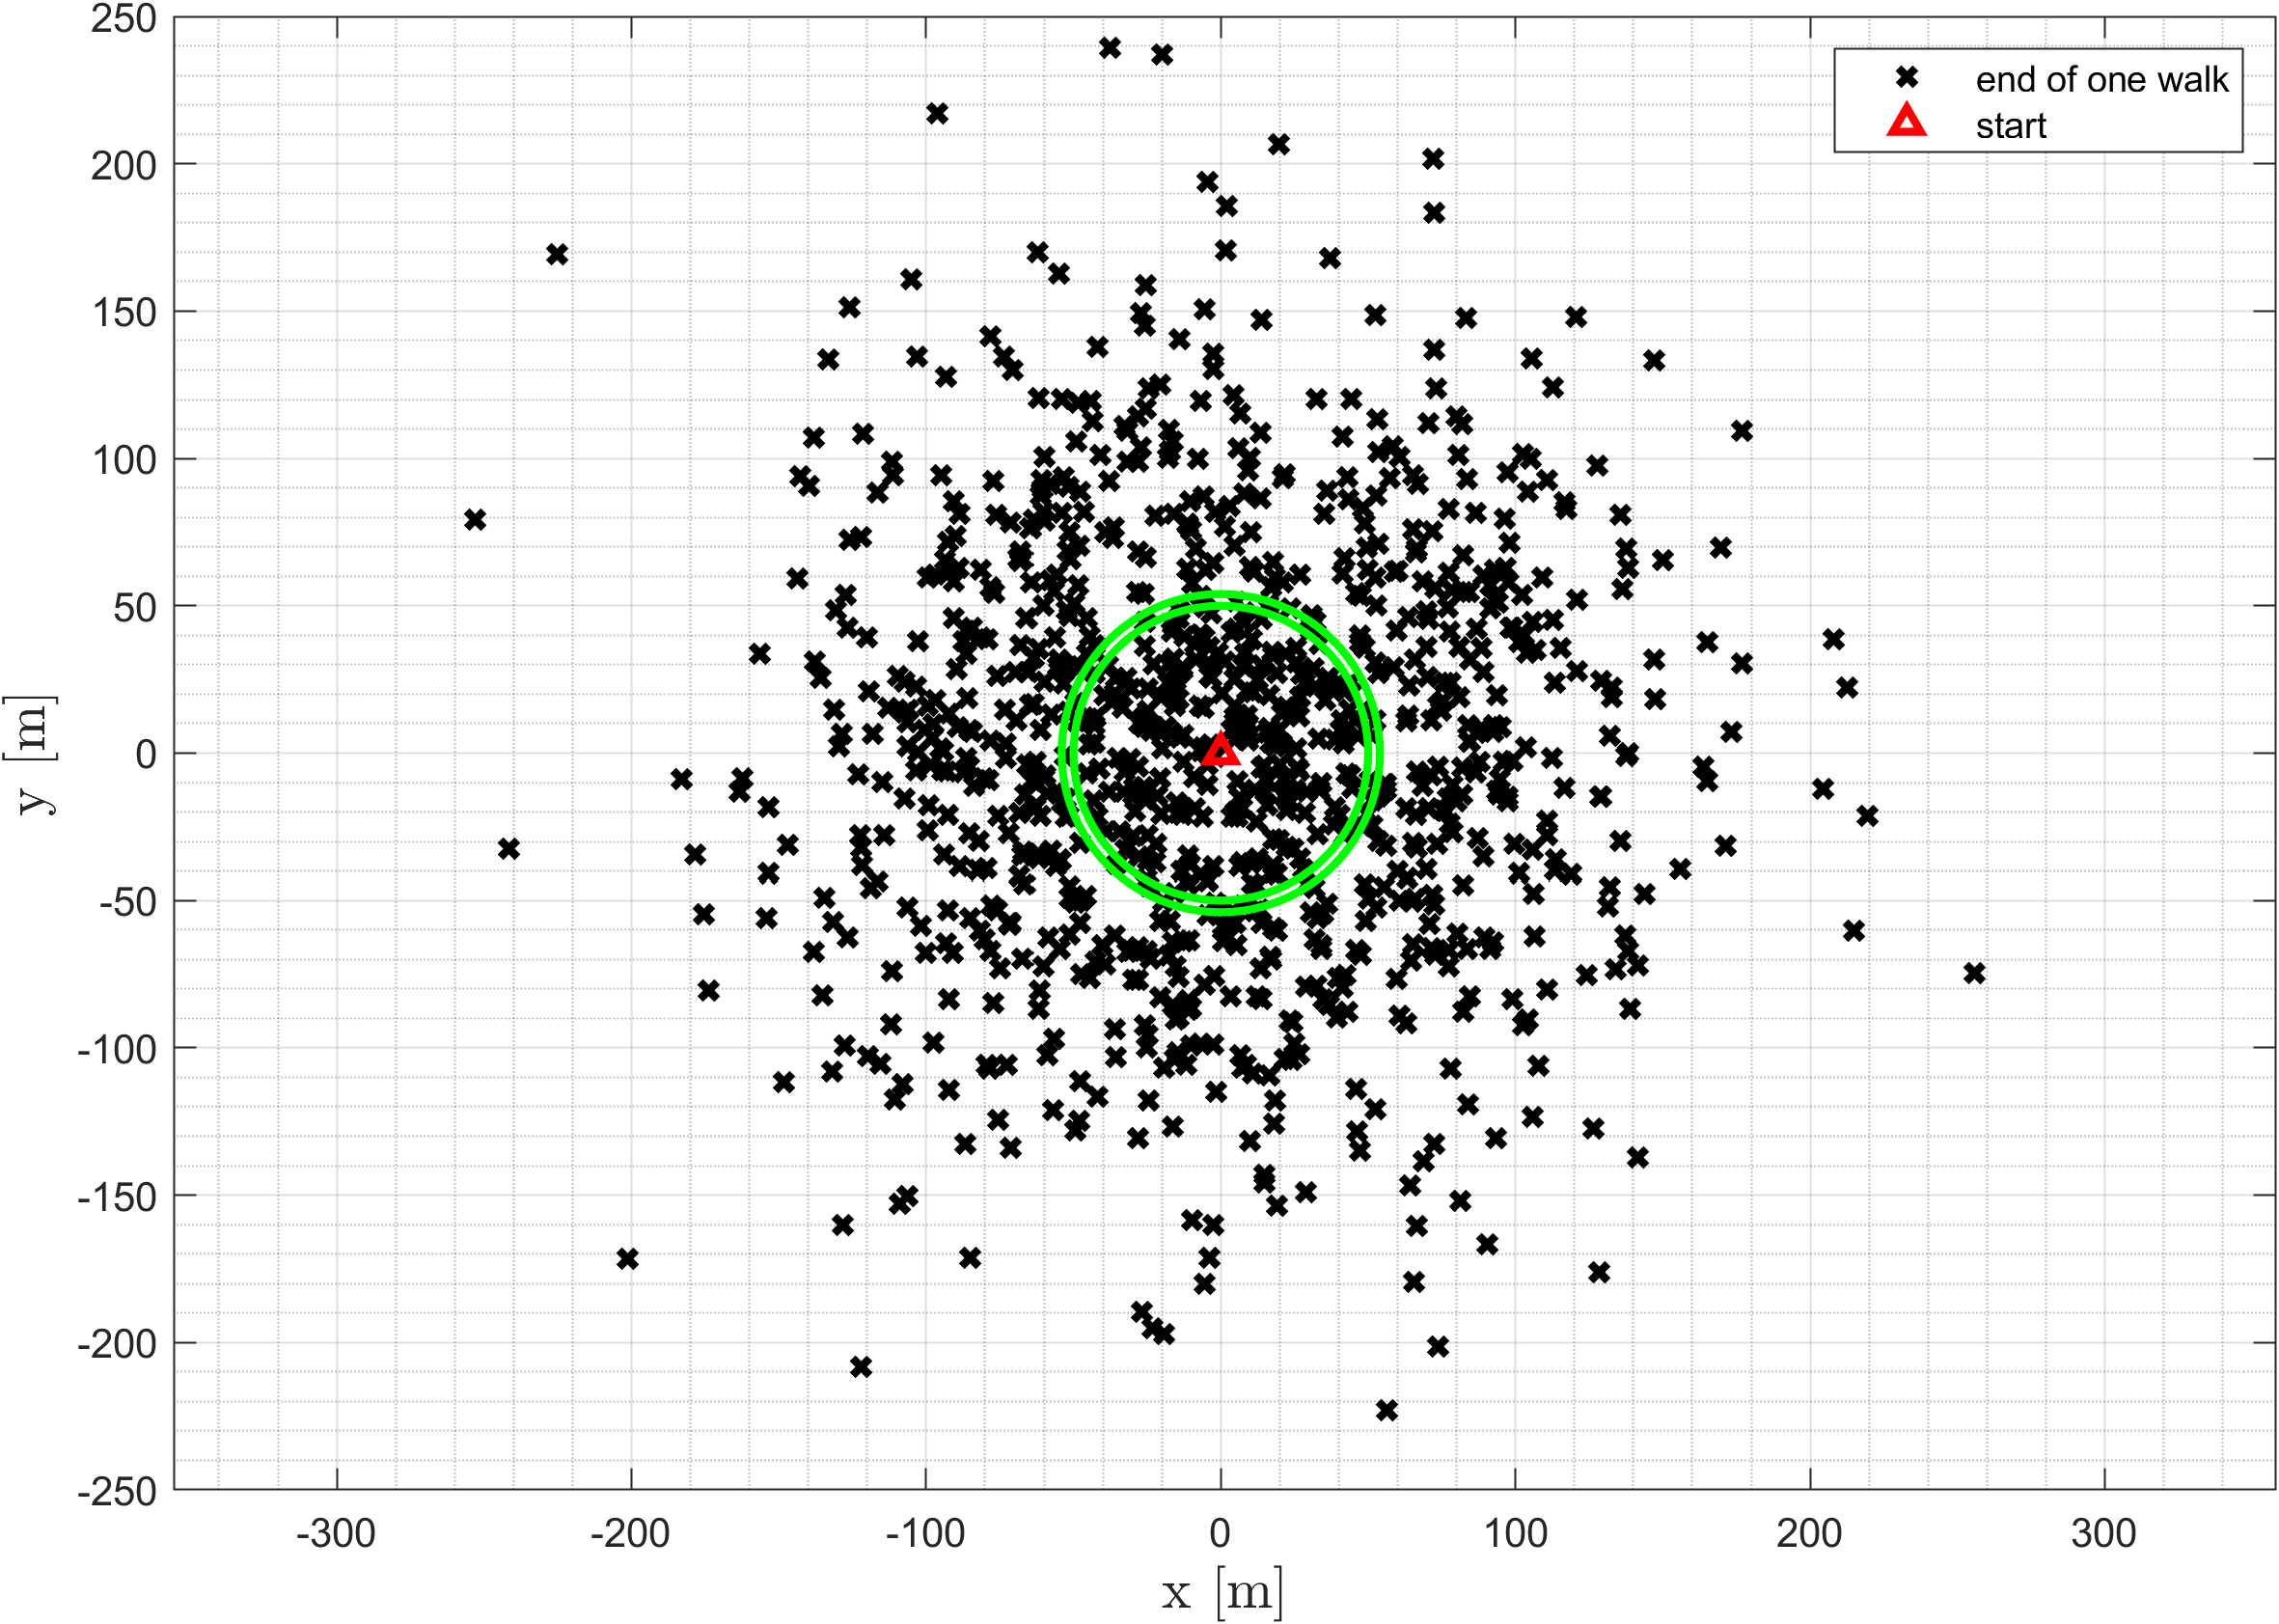
\includegraphics[width=\textwidth]{images/graph1.png}
    \caption{Calculating PDF}
    \label{fig: calculating pdf}
\end{figure}
\noindent Lord Rayleigh's result for the ensemble PDF is:
\begin{equation}
    \displaystyle\frac{2}{n}re^{-\frac{r^2}{n}}
\end{equation}
\begin{itemize}
    \item for a step of $1[m]$
\end{itemize}
\noindent We calculated the PDF function as a function of $r$ for different numbers of realizations and compared the difference between the calculated PDF and Rayleigh's equation. The RMS is calculated by:
\begin{equation}
    RMS=\sqrt{\displaystyle\sum_{r=0}^{r_{max}}\left[PDF_{analytical}\left(r\right)-PDF_{numerical}\left(r\right)\right]^2}
\end{equation}
\begin{figure}[H]
    \centering
    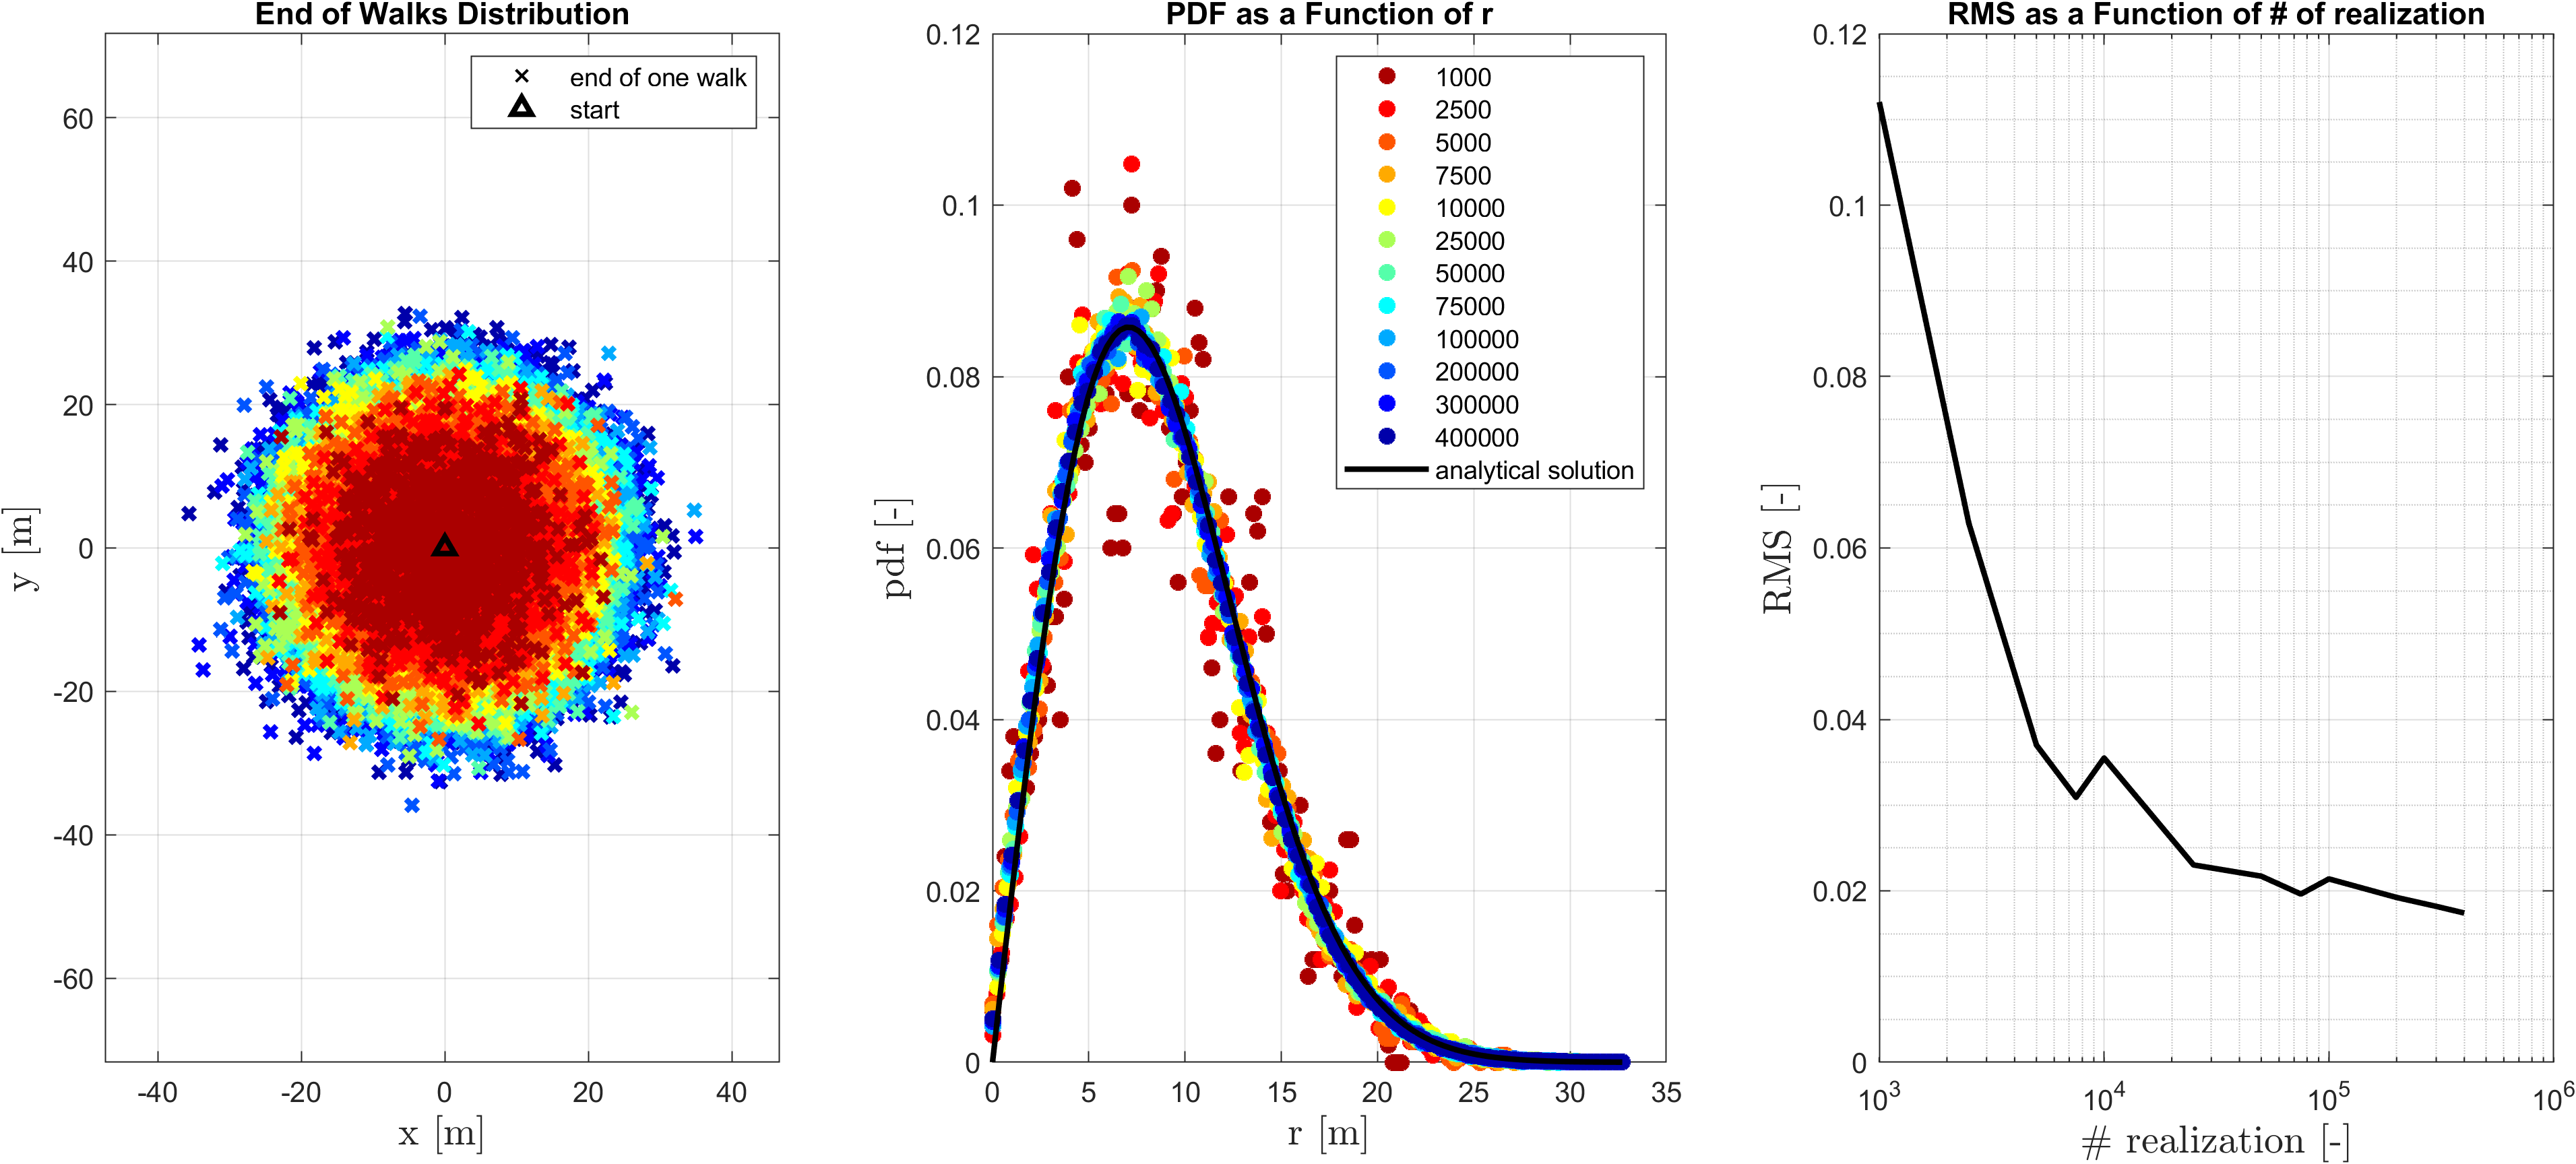
\includegraphics[width=\textwidth]{images/graph2.png}
    \caption{PDF function as a function of realizations}
    \label{fig: pdf for different realizations}
\end{figure}
\noindent We can see that for number of realizations bigger then $10^5$, we can see that the RMS between the calculated PDF and Rayleigh's equation is small enough to consider converged. 

\subsection{Average Displacement}
From the lectures, the average displacement $\langle r\rangle$:
\begin{equation}
    \langle r\rangle=\mathbb{E}\left(r\right)=\int_{-\infty}^\infty{r\cdot PDF\left(r\right)dr}
\end{equation}
Hence, the average displacement as a function of number of realizations is:
\begin{figure}[H]
    \centering
    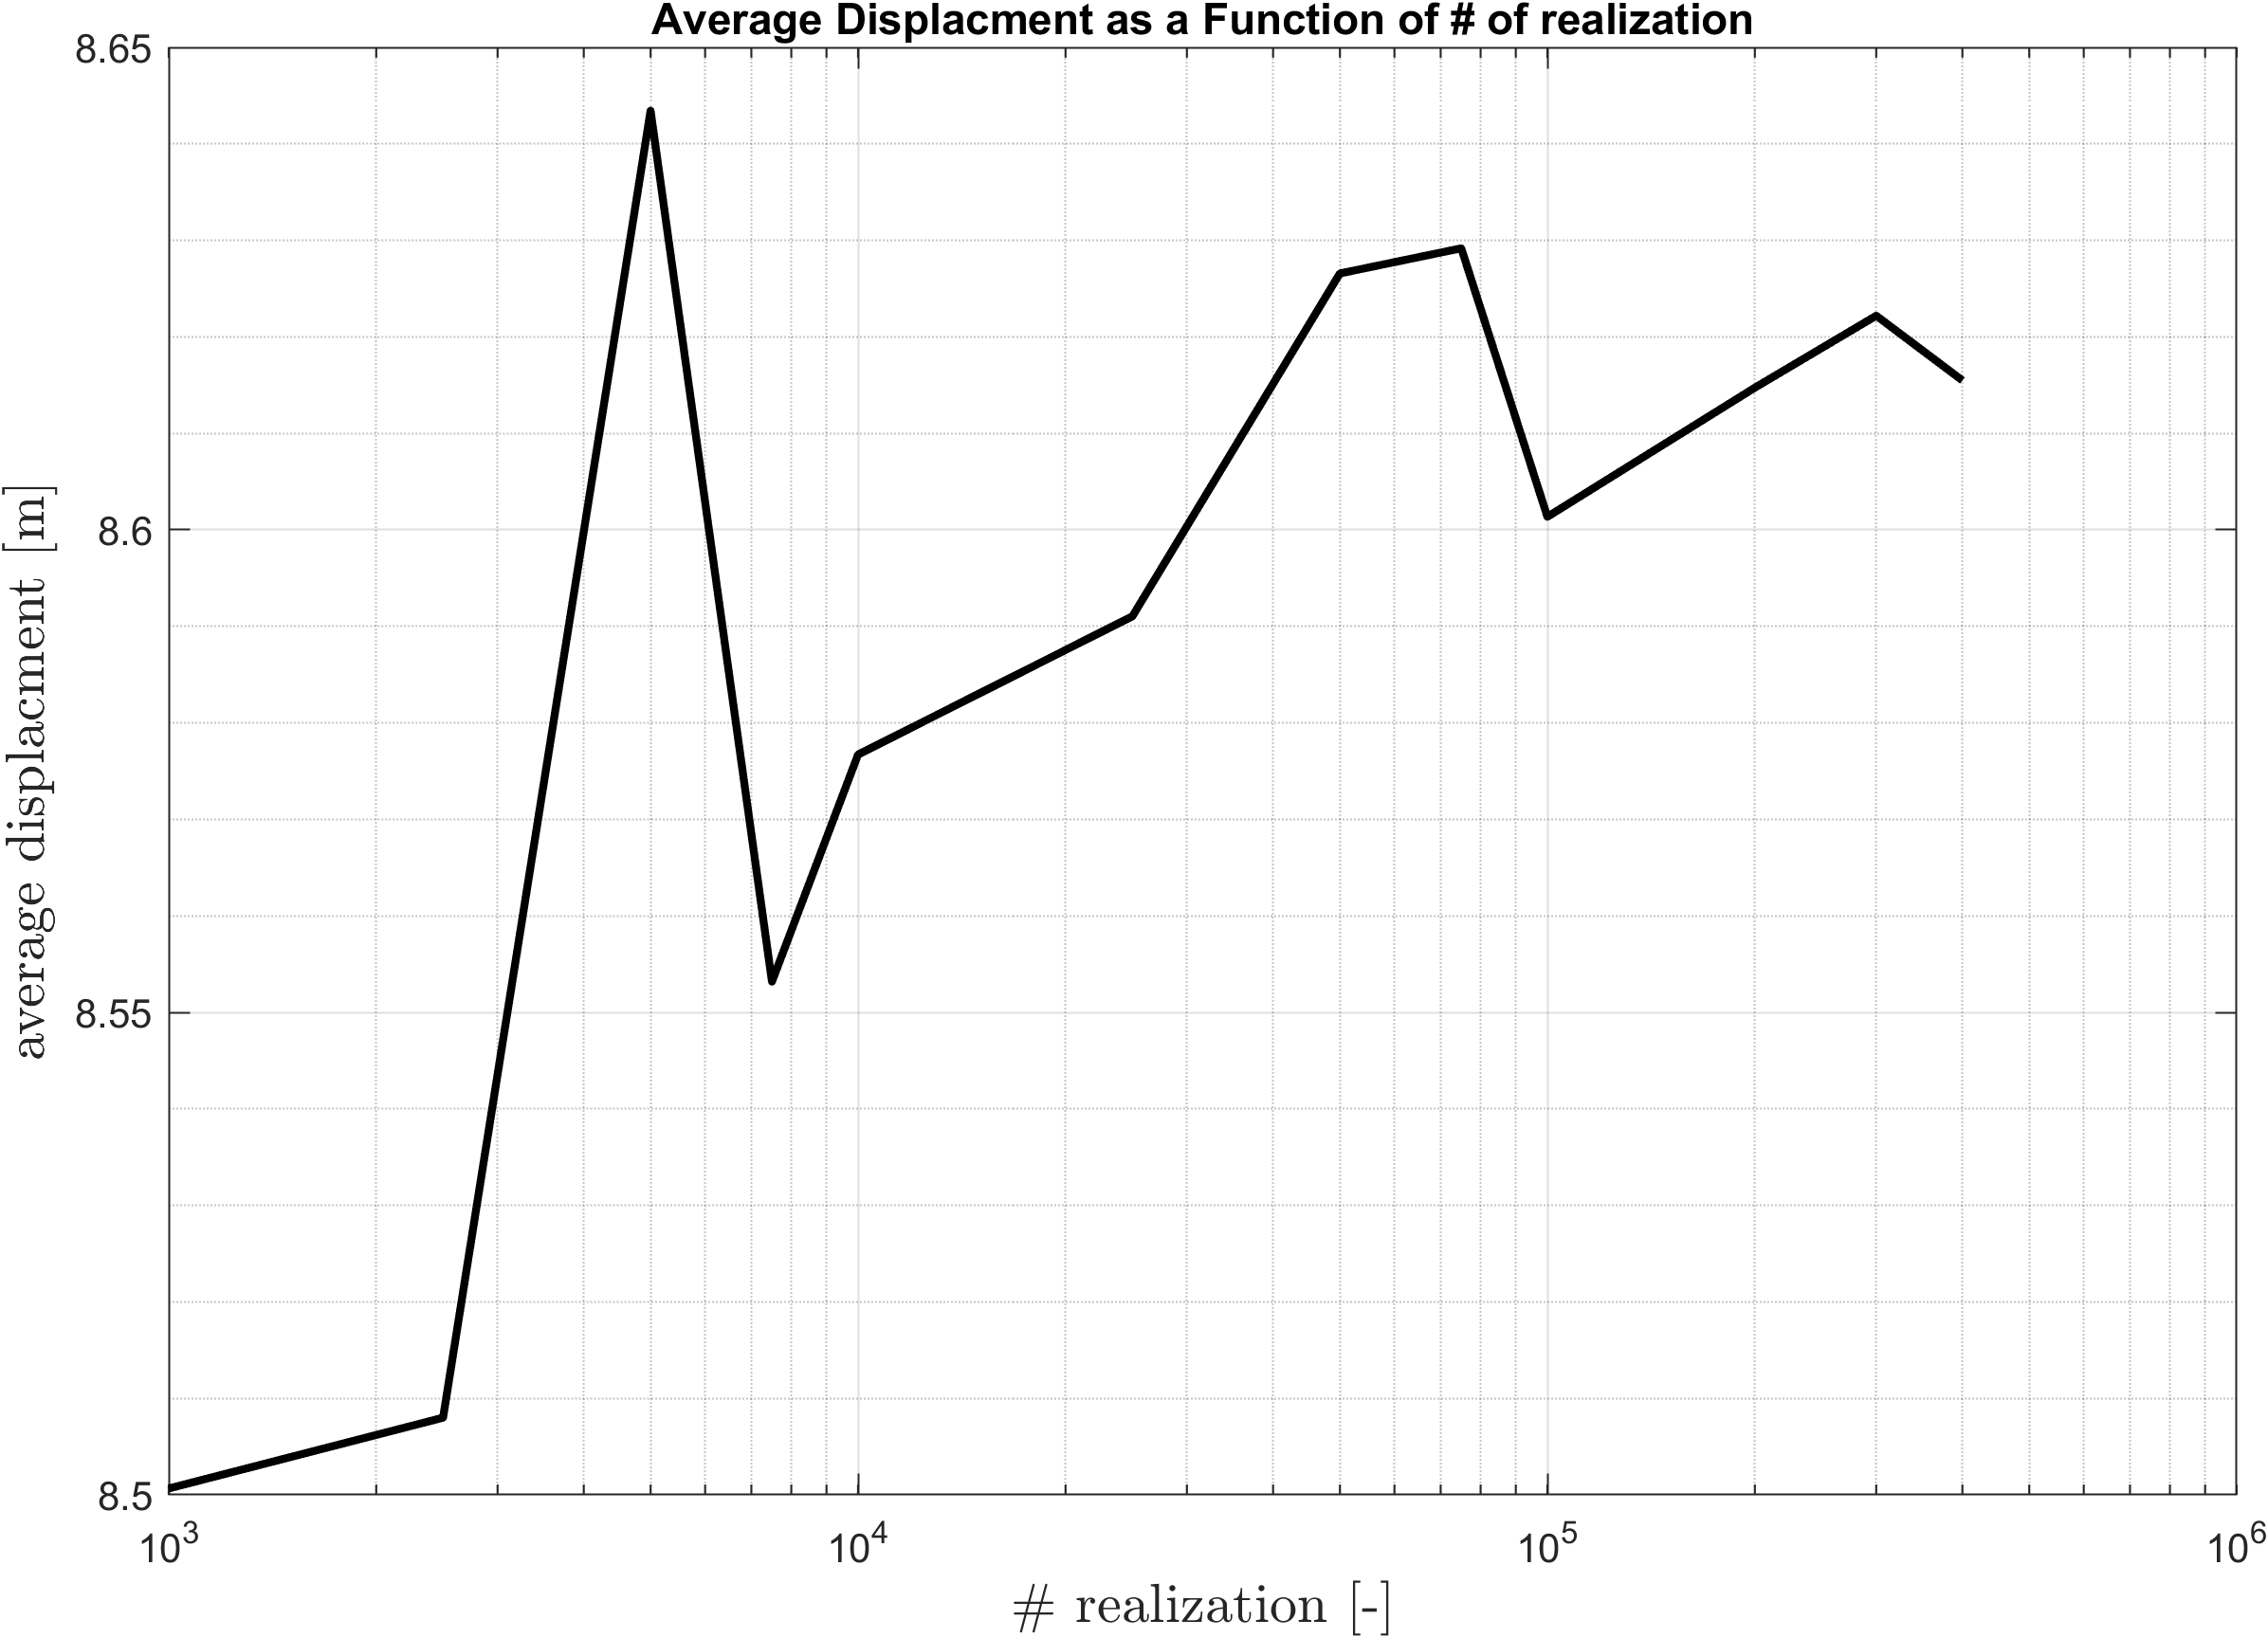
\includegraphics[width=0.8\textwidth]{images/graph3.png}
    \caption{Average Displacement as a function of realizations}
    \label{fig: average displacement as a function of realizations}
\end{figure}
\noindent We can see that the average displacement converge to a value between 8.6 and 8.65.

\subsection{Autocovariance and Autocorrelation}
The covariance is calculated using the \emph{cov} function in \emph{MatLab}. The autocorrelation is the normalized autocovariance. The definition of the covariance is:
\begin{equation}
    Q_{uv}=\mathbb{E}\left[\left(u-\mu_u\right)\left(v-\mu_v\right)\right]
\end{equation}
The autocovariance is therefore:
\begin{equation}
    Q\left(\Delta\ell\right)=\mathbb{E}\left[\left(r\left(\ell\right)-\mu\right)\left(r\left(\ell+\Delta\ell\right)-\mu\right)\right]
\end{equation}
and the autocorrelation is:
\begin{equation}
    R\left(\Delta\ell\right)=\frac{Q\left(\Delta\ell\right)}{\max\left\{Q\left(\Delta\ell\right)\right\}}
\end{equation}
\begin{figure}[H]
    \centering
    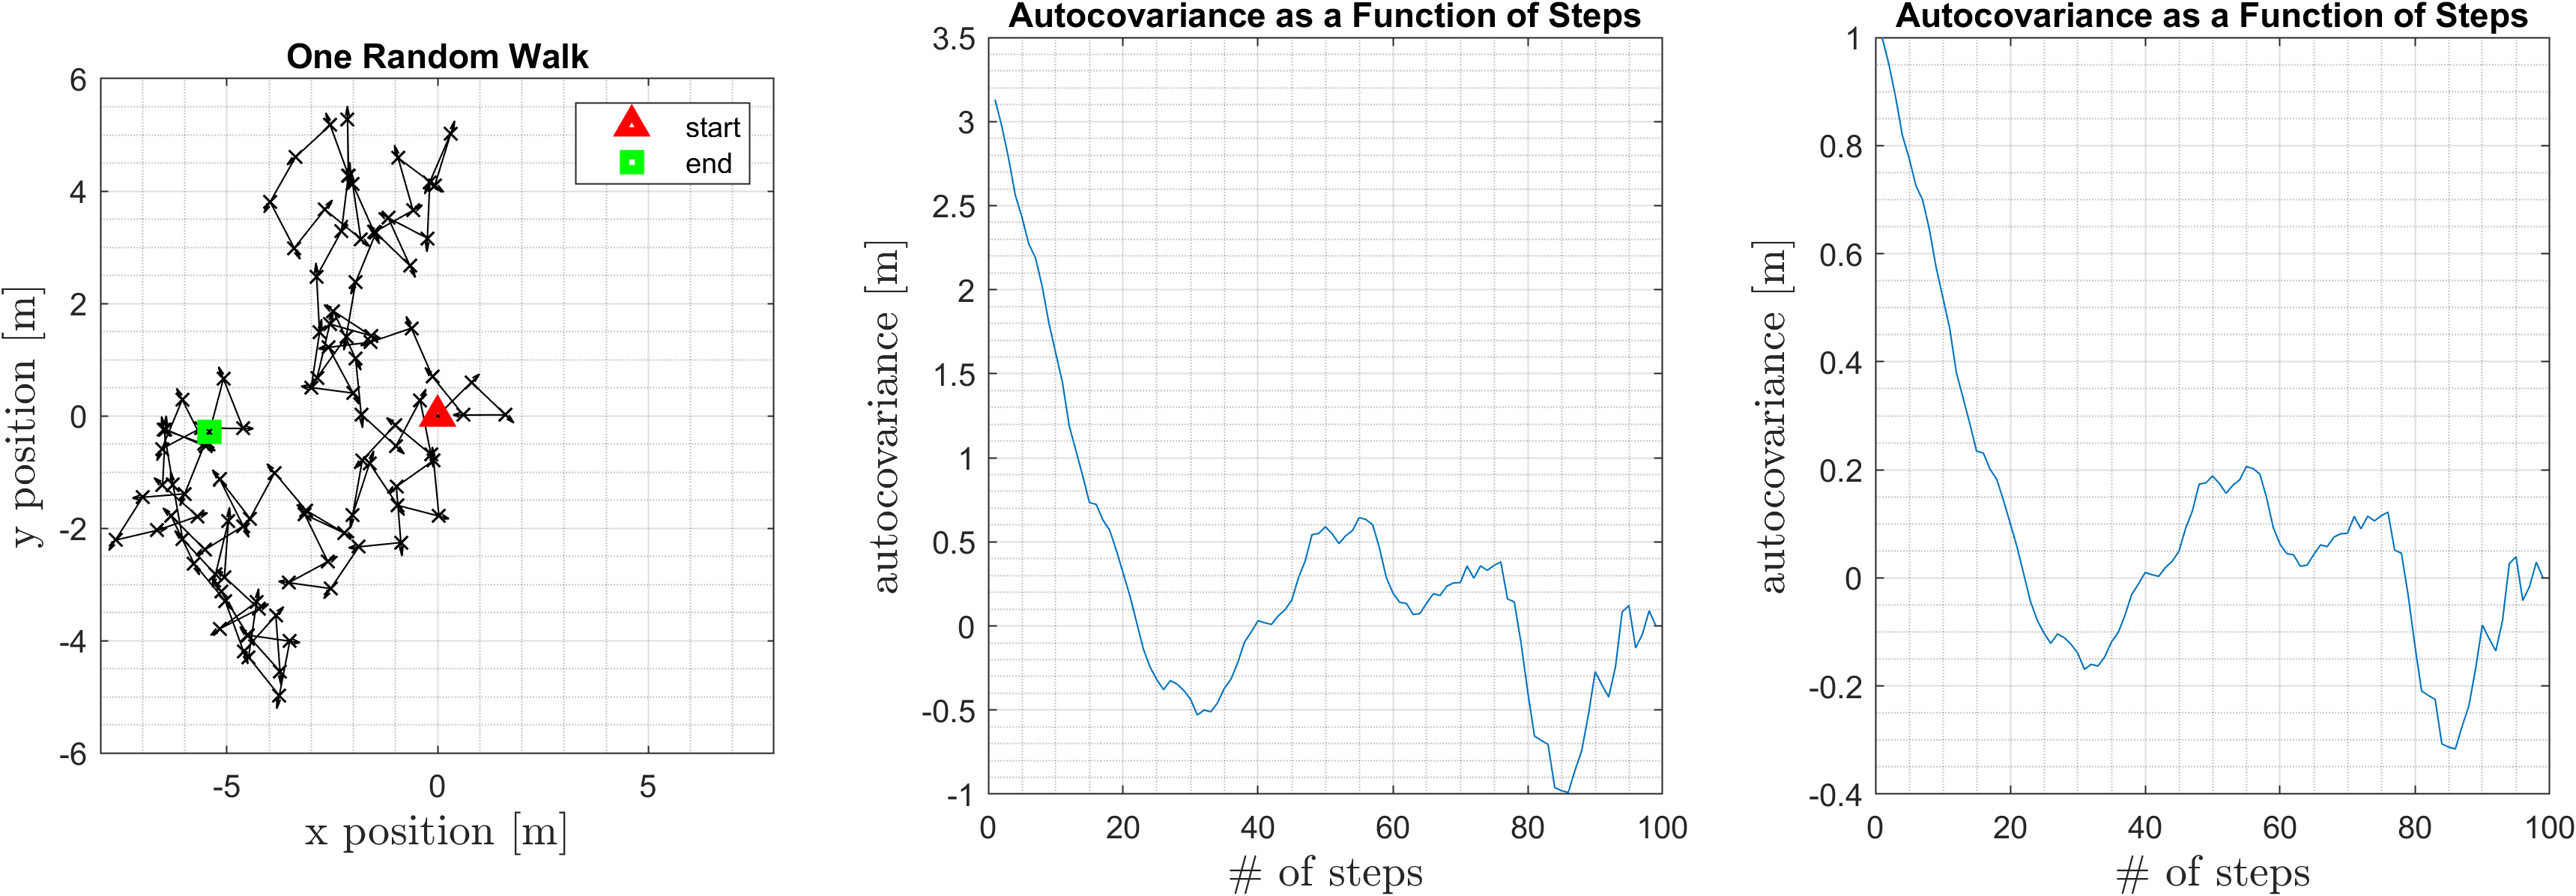
\includegraphics[width=\textwidth]{images/graph4.png}
    \caption{Autocovariance and Autocorrelation}
    \label{fig: autocovariance and autocorrelation}
\end{figure}
\noindent In order to determine how many walks are needed in the ensemble for the autocorrelation to converge we will calculate the autocorrelation over a range of realizations:
\begin{figure}[H]
    \centering
    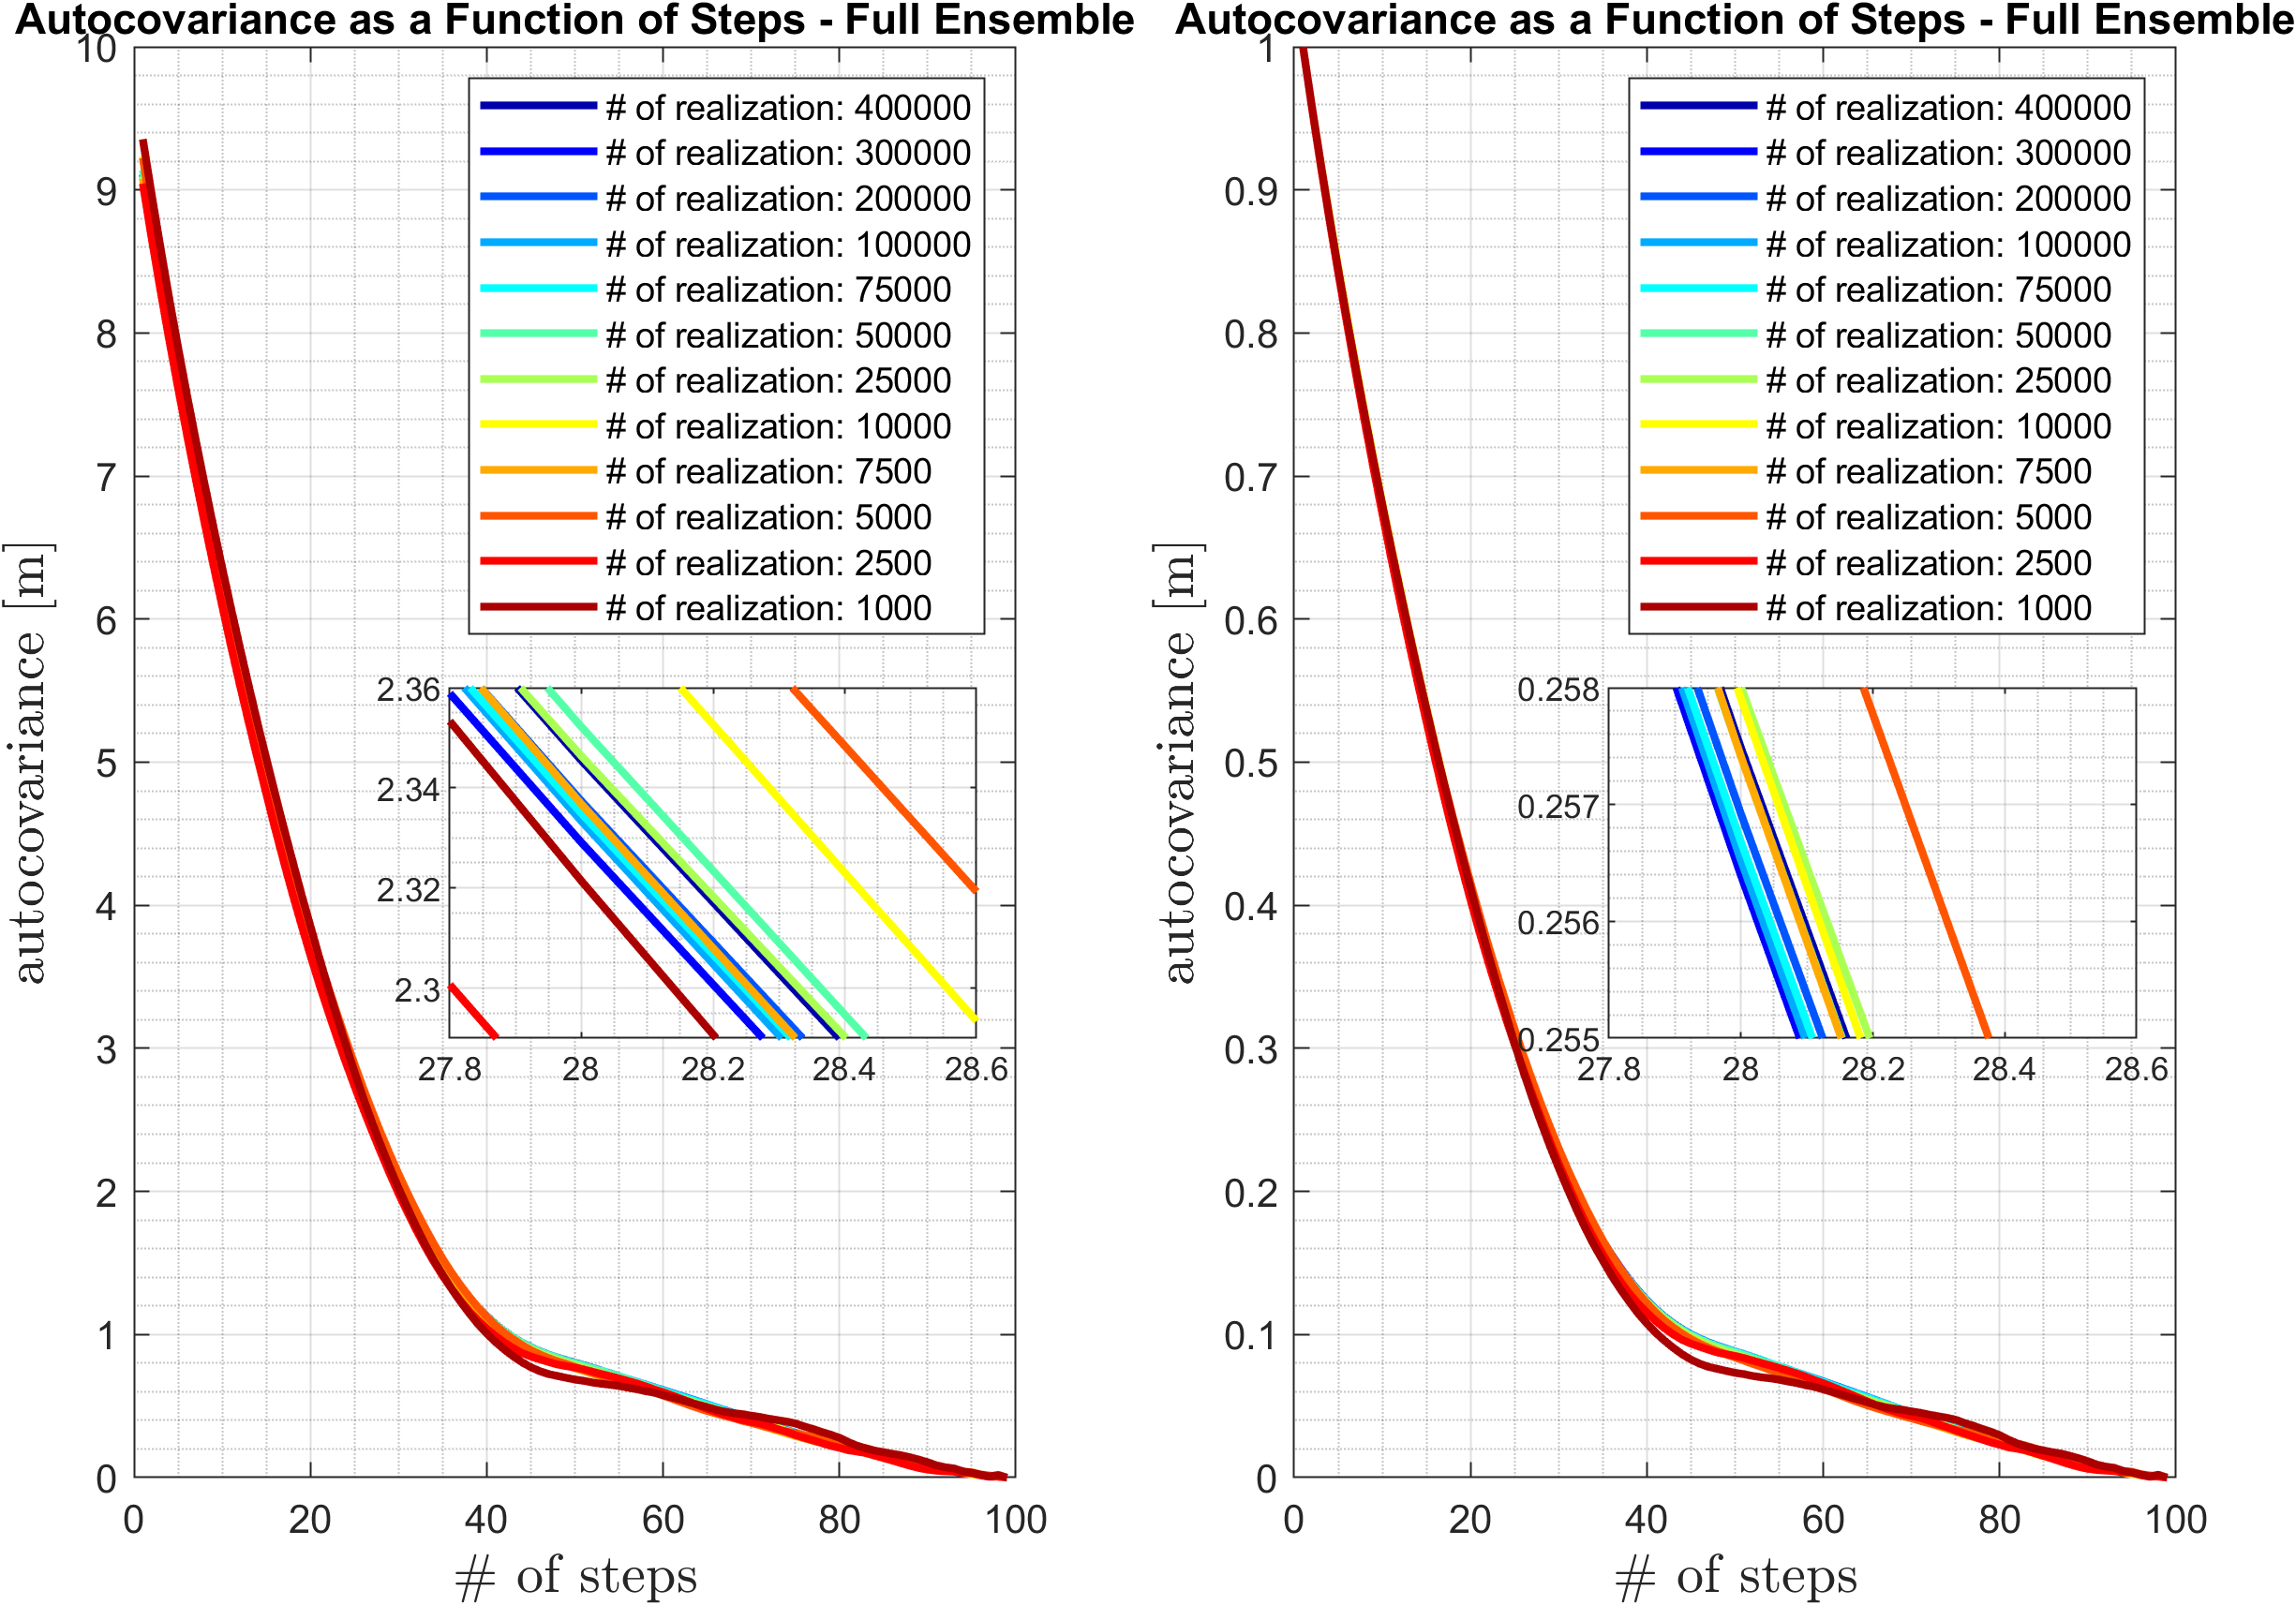
\includegraphics[width=0.7\textwidth]{images/graph5.png}
    \caption{Autocovariance and Autocorrelation ensemble}
    \label{fig: autocovariance and autocorrelation ensemble}
\end{figure}
\noindent We can see that for more that $10^4$ realizations, the autocovariance does not have any significant changes. \\
\underline{I finished this quistion in 3 day}

\newpage
\bibliographystyle{ieeetr}
\bibliography{references}

\newpage
\appendix
\section{Listing of The Computer Program}
\subsection{Q1}
\begin{lstinputlisting}[captionpos=b,stringstyle=\color{magenta},frame=single, numbers=left, style=MatLab-editor, basicstyle=\mlttfamily\small, caption={Code for Q1},mlshowsectionrules=true]{./matlab_code/Q1.m}
\end{lstinputlisting}

\subsection{Q2}
\begin{lstinputlisting}[captionpos=b,stringstyle=\color{magenta},frame=single, numbers=left, style=MatLab-editor, basicstyle=\mlttfamily\small, caption={Code for Q2},mlshowsectionrules=true]{./matlab_code/Q2.m}
\end{lstinputlisting}

\subsection{Q3}
\begin{lstinputlisting}[captionpos=b,stringstyle=\color{magenta},frame=single, numbers=left, style=MatLab-editor, basicstyle=\mlttfamily\small, caption={Code for Q3},mlshowsectionrules=true]{./matlab_code/Q3.m}
\end{lstinputlisting}

\end{document}
